\section{球径による高速化への影響}
\label{sec:diameter}
先行研究より拡張した領域における球径による影響を考えるため,直径を変化させた鋼球を用いて落下球実験を行った.実験条件を,Table.\ref{table:exp-conditions-dia}に示す.それぞれの質量濃度の場合に分けて球径による影響の検討を行う.

\subsection{PAA1.0wt.\%の場合}
PAA1.0wt.\%における球径変化の実験結果をFig.\ref{fig:diameter}に示す.その結果より,落下球の直径と終端速度の関係をFig.\ref{fig:diaUT}(a)に示す.落下球の直径が大きくなると,終端速度が指数関数的に高速化した.また,直径と超音波照射による高速化度合の関係をFig.\ref{fig:diaUT}(b)に示す.落下球の直径10mmをピークとして超音波照射による高速化が見られた.

これらより,式(\ref{eq:Udiff})を用いて整理した結果をFig.\ref{fig:muUdiff}に示す.Fig.\ref{fig:muUdiff}(a)においては先行研究である岩室\cite{ref:8}の実験結果全範囲を,Fig.\ref{fig:muUdiff}(b)においては今回の実験結果によって得られた範囲を拡大した結果を示す.落下球の直径10mm以上において,粘度比と音響境界層を球の半径で規格化した値は,超音波照射による球の高速化度合いに対して正の相関関係にあった.一方で先行研究において示されていた範囲においては,高速化が抑制され非常に小さな値となっていた.この要因として,先行研究である岩室\cite{ref:8}において弾性による影響が示唆されている.本研究\ref{sec:elasticity-discussion}章にて,それらの議論を行う.

\begin{figure}[ht]
    \centering
    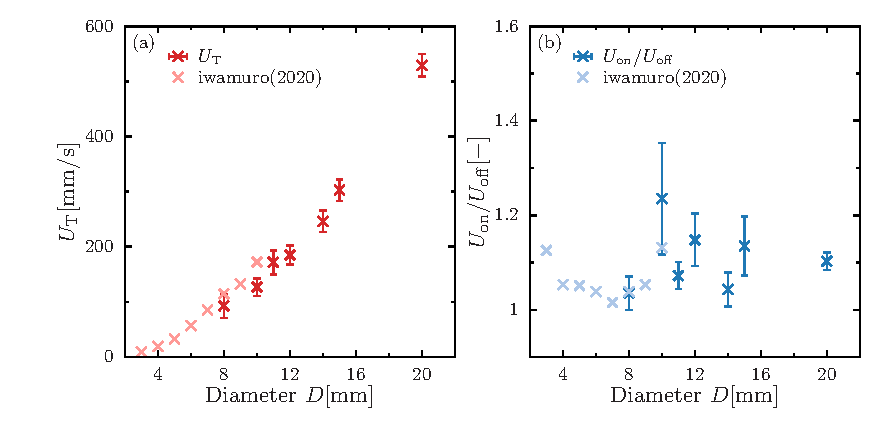
\includegraphics[width=1\textwidth]{./5-Results/diaUT_Udiff.eps}
    \caption{Relationship between diameter and (a)terminal velocity, (b)velocity rato.}
    \label{fig:diaUT}
\end{figure}

\begin{figure}[ht]
    \centering
    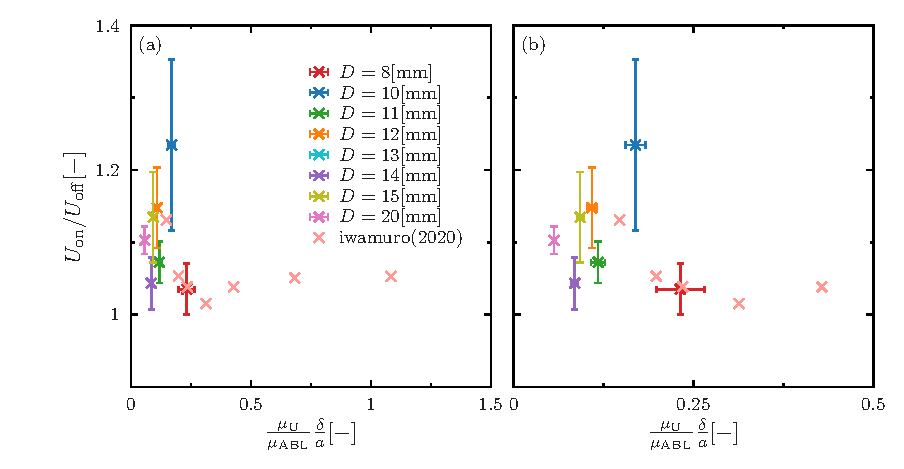
\includegraphics[width=1\textwidth]{./5-Results/mu_Udiff.eps}
    \caption{Relationship between velocity rato and viscosity ratio, the acoustic boundary layer thickness, radius (a)with Iwamuro (2020), (b)without Iwamuro (2020).}
    \label{fig:muUdiff}
\end{figure}

\newpage

\subsection{PAA0.5wt.\%の場合}
PAA0.5wt.\%における球径変化の実験結果をFig.\ref{fig:diameter-0.5}に示す.その結果より,落下球の直径と終端速度の関係をFig.\ref{fig:diaUT0.5}(a)に示す.落下球の直径が大きくなると,PAA1wt.\%の場合と同様に終端速度が指数関数的に高速化した.また,直径と超音波照射による高速化度合いの関係をFig.\ref{fig:diaUT0.5}(b)に示す.PAA1wt.\%の場合と同様に落下球の直径10mmをピークとして超音波照射による高速化が見られた.

式(\ref{eq:Udiff})を用いて高速化度合を整理した結果をFig.\ref{fig:muUdiff0.5}に示す.落下球の直径が10mm以上において粘度比と音響境界層を球の半径で規格化した値は,超音波照射による球の高速化度合いに対して正の相関関係にあった.一方で,落下球の直径5mmは高速化度合いが非常に小さくなった.このことに関して,他の結果も含めて,本研究\ref{sec:viscosity},\ref{sec:elasticity-discussion}章にて,議論を行う.
\begin{figure}[ht]
    \centering
    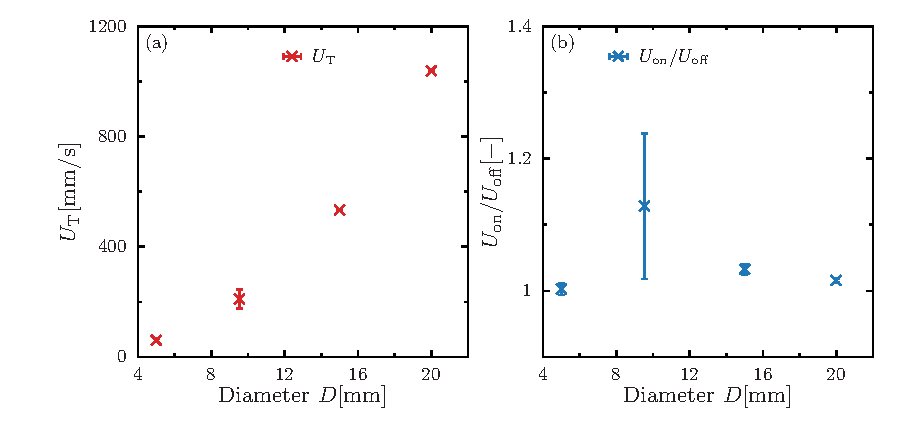
\includegraphics[width=1\textwidth]{./5-Results/diameter-0.5/diaUT_Udiff.eps}
    \caption{Relationship between diameter and (a)terminal velocity, (b)velocity rato.}
    \label{fig:diaUT0.5}
\end{figure}

\begin{figure}[ht]
    \centering
    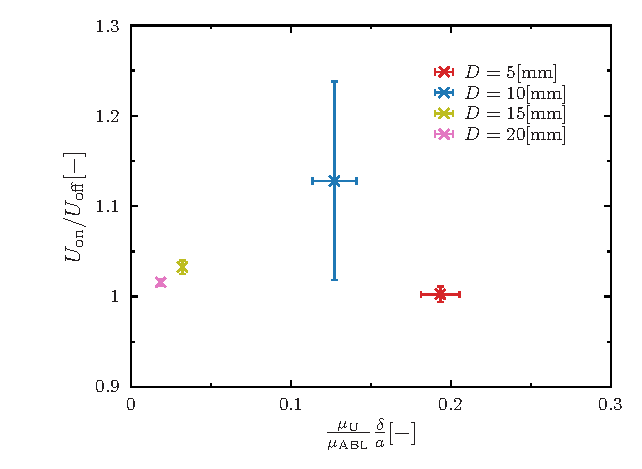
\includegraphics[width=0.8\textwidth]{./5-Results/diameter-0.5/mu_Udiff.eps}
    \caption{Relationship between velocity rato and viscosity ratio, the acoustic boundary layer thickness, radius.}
    \label{fig:muUdiff0.5}
\end{figure}

\clearpage

\subsection{PAA0.2,1.3wt.\%の場合}
PAA0.2,1.3wt.\%における球径変化の実験結果をFig.\ref{fig:diameter-0.2-1.3}に示す.その結果より,落下球の直径と終端速度の関係をFig.\ref{fig:diaUT0.2-1.3}(a)に示す.落下球の直径が大きくなると,他の質量濃度と同様に終端速度が高速化した.また,直径と超音波照射による高速化度合いの関係をFig.\ref{fig:diaUT0.2-1.3}(b)に示す.PAA0.2wt.\%において,顕著な高速化は見られなかった.一方で,PAA1.3wt.\%において,落下球の直径が小さい場合に高速化が見られた.

式(\ref{eq:Udiff})を用いて高速化度合いを整理した結果をFig.\ref{fig:muUdiff0.2-1.3}に示す.粘度比と音響境界層厚さを球の半径で規格化した値は,超音波照射による球の高速化度合いに対して正の相関関係にあった.他の結果も含めて,本研究\ref{sec:viscosity},\ref{sec:elasticity-discussion}章にて,より詳しい議論を行う.

\begin{figure}[ht]
    \centering
    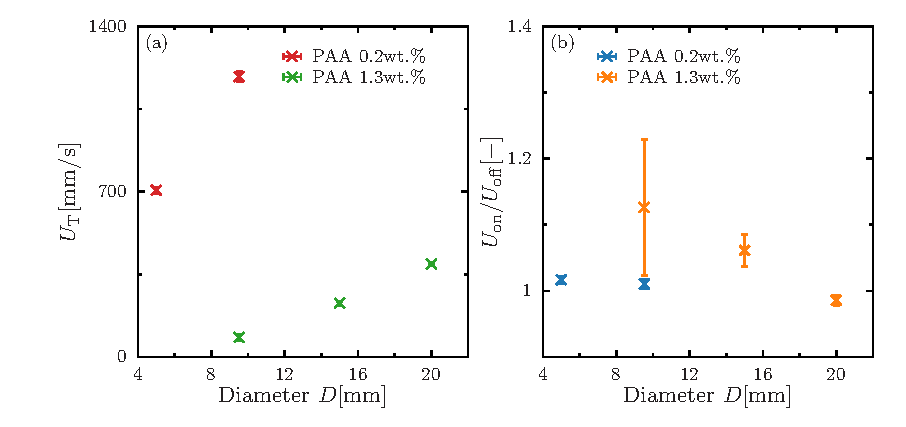
\includegraphics[width=0.9\textwidth]{./5-Results/diameter-0.2-1.3/diaUT_Udiff.eps}
    \caption{Relationship between diameter and (a)terminal velocity, (b)velocity rato.}
    \label{fig:diaUT0.2-1.3}
\end{figure}

\begin{figure}[ht]
    \centering
    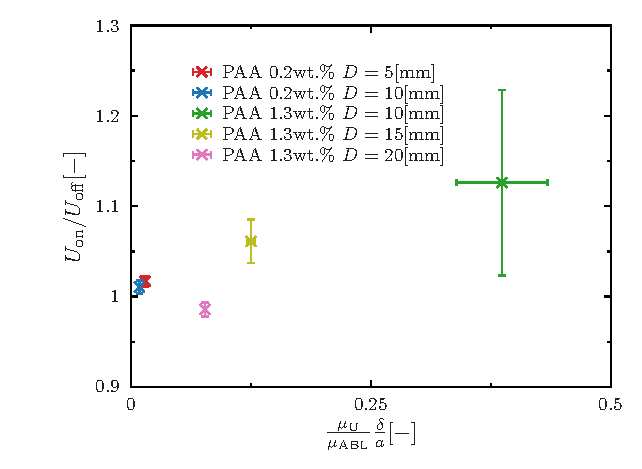
\includegraphics[width=0.7\textwidth]{./5-Results/diameter-0.2-1.3/mu_Udiff.eps}
    \caption{Relationship between velocity rato and viscosity ratio, the acoustic boundary layer thickness, radius.}
    \label{fig:muUdiff0.2-1.3}
\end{figure}